\section{Протокол и модель злоумышленника}

Модель протокола и злоумышленника, которую мы описываем далее, расширяет стандартные модели для (автоматического) анализа протоколов безопасности
\cite{Amadio2002} в двух отношениях. Во-первых, сообщения могут строиться с помощью
оператора $Exp(\cdot,\cdot)$, означающего экспоненциацию, и оператора произведения "\(\cdot\)". Во‑вторых, помимо стандартных правил перезаписи
модели Долева–Яо, злоумышленник снабжён дополнительными «правилами-оракулами», которые будут конкретизированы правилами экспоненциации термов.
В дальнейшем мы приведём формальное определение нашей модели, задав терминологию для термов, сообщений, протоколов, злоумышленника и атак.

\subsection{Термины и сообщения}

Множество термов \textit{term} определяется следующей грамматикой:
\[
\begin{array}{rl}
  \mathit{term} ::= & \mathcal{A} \mid \mathcal{V} \mid (\mathit{term}, \mathit{term}) \mid \{\mathit{term}\}^{s}_{k_{\mathit{term}}} \\
                  & \mid \{\mathit{term}\}^{p}_{k} \mid \mathit{Exp}(\mathit{term}, \mathit{product}) \\
\mathit{product} ::= & \mathit{term}^{\mathbb{Z}} \mid \mathit{term}^{\mathbb{Z}} \cdot \mathit{product}
\end{array}
\]
где $\mathcal{A}$ — конечное множество констант (атомарных сообщений), включающее имена субъектов, случайные значения, ключи, и специальные
константы $1$ и секрет. Множество $\mathcal{K} \subseteq \mathcal{A}$ содержит все открытые и закрытые ключи. $\mathcal{V}$ — конечное
множество переменных, $\mathbb{Z}$ — множество целых чисел, используется для показателей в произведениях. Предполагается, что существует биекция
${.}^{-1} : \mathcal{K} \to \mathcal{K}$, сопоставляющая каждому открытому (закрытому) ключу $k$ соответствующий закрытый (открытый) $k^{-1}$.

Бинарный символ $\langle\cdot,\cdot\rangle$ обозначает объединение в пару, символ $\{\cdot\}^{s}$ используется для симметричного шифрования,
а символ $\{\cdot\}^{p}$ — для шифрования с открытым ключом. Заметим, что симметричный ключ может быть произвольным термом, в то время как для
шифрования с открытым ключом допускаются только атомарные ключи из $\mathcal{K}$.

Оператор произведения ``$\cdot$'' моделирует умножение в абелевой группе. Например, произведение $a^2 \cdot b^3 \cdot c^{-2}$ представляет элемент
этой группы, где $a^2 = a \cdot a$, $b^3 = b \cdot b \cdot b$, а $c^{-2} = c^{-1} \cdot c^{-1}$, причём $c^{-1}$ — обратный к $c$. В протоколе
A-GDH.2, к примеру, в качестве абелевой группы используется подгруппа $G$ порядка $q$ мультипликативной группы $\mathbb{Z}_p^*$, где $p$ и $q$
— простые числа. Термы и продукты рассматриваются с учётом коммутативности и ассоциативности оператора $\cdot$, а также с учётом тождества $t^1
= t$. Например, термы $d^1 \cdot c^{-2} \cdot (b^3 \cdot a^2) \quad \text{и} \quad a^2 \cdot b^3 \cdot c^{-2} \cdot d$ считаются представлениями
одного и того же продукта. Также, если мы пишем $t_1^{z_1} \cdots t_n^{z_n}$, то всегда предполагается, что ведущий символ $t_i$ не является
продуктом. Этого можно достичь, расставив скобки соответствующим образом. Мы используем обозначение $t_1^{z_1} \cdots t_n^{z_n}$ для обозначения
продукта, где $z_i$ — некоторые ненулевые целые числа. Оператор $\mathit{Exp}(\cdot,\cdot)$ означает возведение в степень. Например,
$\mathit{Exp}(a, b^2 \cdot c^{-1}) = a^{b^2 \cdot c^{-1}}$.

Если $t, t_1, \dots, t_n$ — термы и $n \geq 2$, то произведение вида $t^z$ (при $z \ne 1$) или вида $t_1^{z_1} \cdots t_n^{z_n}$ называется
\textit{нестандартным термом} (non-standard term). Мы часто обозначаем терм или продукт как \textit{терм}. Чтобы различать их, мы используем
понятие \textit{стандартного терма}, противопоставляя его нестандартному.

Переменные обозначаются $x,y,\dots$, а сами термы — $s,t,u,v$. 
Конечные множества термов пишем $E,F,\dots$ и их «украшенные» варианты.  
Для краткости будем записывать $E\cup F \;\text{как}\; E,F, \text{объединение} E\cup\{t\} \;\text{как}\; E,t, \text{и} E\setminus\{t\} \;\text{как}\; E\setminus t$.

Для терма $t$ и множества термов $E$ через $\mathcal{V}(t)$ и $\mathcal{V}(E)$ обозначим
соответственно множество переменных, встречающихся в $t$ и в $E$.

Наземный терм (или \emph{сообщение}) — это терм без переменных.
Термины \emph{стандартное} и \emph{нестандартное сообщение} употребляются
так же, как стандартный и нестандартный терм.  
\emph{(Наземная) подстановка} $\sigma$ — это отображение из $\mathcal V$ в множество
стандартных наземных термов.  Применение $\sigma$ к терму $t$ (или множеству $E$)
обозначается $t\sigma$ (соответственно $E\sigma$) и определяется обычным образом.

Скажем, что термы $t$ и $t'$ \emph{совпадают с точностью до показателей произведения}
(пишем $t\approx t'$), если они различаются только значениями степеней.  Например:
\[
\begin{aligned}
\langle Exp(g,a^{2}),\; Exp(g,b^{-3}\!\cdot c) \rangle
&\;\approx\;
\langle Exp(g,a^{0}),\; Exp(g,b^{2}\!\cdot c^{5}) \rangle \\[2pt]
&\not\approx\;
\langle Exp(g,b^{1}),\; Exp(g,a^{2}\!\cdot c^{5}) \rangle
\end{aligned}
\]
Отношение естественно расширяется на подстановки:
$\sigma\approx\sigma'$ тогда и только тогда, когда
$\sigma(x)\approx\sigma'(x)$ для любой переменной $x$.

Пусть $u$ — стандартный терм, а $v$ — произвольный терм.
\emph{Замена} $\delta=[u\!\mapsto\! v]$ отправляет любой терм $t$
в терм $t\delta=t[u\!\leftarrow\! v]$, полученный заменой всех
вхождений $u$ на $v$.

\begin{definition}
Применение замены $\delta=[v\!\mapsfrom\! u]$ к терму $t$ (обозначается $t\delta$)
задаётся индукцией по структуре $t$:
\[
\begin{array}{lcl}
\text{-- If } t = u,               && t\delta = v. \\[2pt]
\text{-- If } t \in \mathcal{A}\cup\mathcal{V},\; t\neq u,
                                && t\delta = t. \\[4pt]
\text{-- If } t = \langle t_{1},t_{2}\rangle,
                                && t\delta = \langle t_{1}\delta,\,t_{2}\delta\rangle. \\[4pt]
\text{-- If } t = \{t_{1}\}^{s}_{k},
                                && t\delta = \{t_{1}\delta\}^{s}_{t_2\delta}. \\[4pt]
\text{-- If } t = \{t_{1}\}^{p}_{k},
                                && t\delta = \{t_{1}\delta\}^{p}_{t_2\delta}. \\[4pt]
\text{-- If } t = Exp\!\bigl(t_{0},\,t_{1}^{z_{1}}\!\cdots t_{p}^{z_{p}}\bigr),
                                && t\delta = Exp\!\bigl(t_{0}\delta,\,(t_{1}\delta)^{z_{1}}\!\cdots(t_{p}\delta)^{z_{p}}\bigr). \\[6pt]
\text{-- If } t = t_{1}^{z_{1}}\!\cdots t_{p}^{z_{p}},
                                && t\delta = (t_{1}\delta)^{z_{1}}\!\cdots (t_{p}\delta)^{z_{p}}.  
\end{array}
\]
\end{definition}

Например, для $\delta=[\!Exp(g,a)\mapsfrom\!1]$ имеем $Exp(g,a^{2})\delta=Exp(g,a^{2}), \text{ и } Exp(g,a\!\cdot\! b)\delta=Exp(g,a\!\cdot\! b)$.
По определению результат $t\delta$ единствен.

Подстановку $\sigma$ можно сочетать с заменой $\delta$:
композиция $\sigma\delta$ даёт подстановку, определяемую правилом
$x(\sigma\delta)=(x\sigma)\delta$ для всех $x\in\mathcal V$.

Множество всех подтермов $S(t)$ определяется так:
\[
\begin{array}{@{\!\!}l@{\quad}l}
\text{-- Если } t \in \mathcal{A} \text{ or } t \in \mathcal{V}, & S(t)=\{t\};\\[4pt]
\text{-- Если } t=\langle u,v\rangle,\; \{u\}^{s}_{v}, \text{ or } \{u\}^{p}_{v}, &
      S(t)=\{t\}\cup S(u)\cup S(v);\\[4pt]
\text{-- Если } t=Exp\!\bigl(u,t_{1}^{z_{1}}\!\cdots t_{p}^{z_{p}}\bigr), &
      S(t)=\{t\}\cup S(u)\cup\displaystyle\bigcup_{i=1}^{p} S(t_i);\\[8pt]
\text{-- Если } t=t_{1}^{z_{1}}\!\cdots t_{p}^{z_{p}}, &
      S(t)=\{t\}\cup\displaystyle\bigcup_{i=1}^{p} S(t_i).
\end{array}
\]
Здесь все $t_{i}$ предполагаются стандартными термами.

Мы полагаем $S(E)=\bigcup_{t\in E} S(t)$. Заметим, что \(\!Exp(a,b^{2}\!\cdot c^{1})\) и \(b^{2}\!\cdot c^{1}\!\cdot d^{1}\)
\emph{не} являются подтермами терма
\(\!Exp(a,b^{2}\!\cdot c^{1}\!\cdot d^{1})\).

Множество \emph{расширенных подтермов} терма \(t\) определим как $S_{\!\text{ext}}(t)=S(t)\cup\{\,M\mid \!Exp(u,M)\in S(t)\}$.
Иными словами, если в \(t\) встречается подтерм вида \(\!Exp(u,M)\),
то сам продукт \(M\) также включается в \(S_{\!\text{ext}}(t)\).

Множество факторов терма \(t\), обозначаемое \(\mathcal{F}(t)\), определяется рекурсивно:

\[
\begin{array}{l}
\text{-- Если $t$ является стандартным и не содержит } \!Exp(\cdot,\cdot), \text{ то }\mathcal{F}(t)=\{t\}.\\[4pt]
\text{-- Если } t=\!Exp(u,t_1^{*}\!\cdots t_p^{*}), \text{ то }\mathcal{F}(t)=\{u,t_1,\dots,t_p\}.\\[4pt]
\text{-- Если } t=t_1^{*}\!\cdots t_p^{*}, \text{ то }\mathcal{F}(t)=\{t_1,\dots,t_p\}.
\end{array}
\]

Заметим, что $\mathcal{F}(t)$ содержит только стандартные термы.  
Например, при $a,b,c \in \mathcal{A}$ имеем $\mathcal{F}\!\bigl(a^{2}\!\cdot b^{1}\!\cdot c^{-1}\bigr)=\{a,b,c\}$.

Рассмотрим два способа измерения «размера» терма. В одном случае учитывается продукт в показателях, в другом — нет.  
В любом случае размер определяется по DAG‑представлению терма:
$|t| \;:=\; \operatorname{Card}\!\bigl(S(t)\bigr) (|t|_{\text{ext}} \;:=\; \operatorname{Card}\!\bigl(S_{\!\text{ext}}(t)\bigr)$,
то есть как количество (расширенных) подтермов $t$.

\medskip
\noindent
\textbf{Замечание 2.2.}\;
Всегда выполняется неравенство $\,|t|_{\text{ext}} \le 2\,|t|$.

\medskip
Определения $|\cdot|$ и $|\cdot|_{\text{ext}}$ не учитывают длину показателей.  
Чтобы измерить объём памяти, необходимый для их хранения, введём
\[
\lVert t\rVert_{\text{exp}} := 
\sum_{\,t_i^{\,z_i}\cdots t_n^{z_n}\in S(t)} |z_i| + \cdots + |z_n|,
\]
где $|z_i|$ — число битов в двоичной записи целого $z_i$.

Полный размер терма определяется как
\[
\lVert t\rVert := |t| + \lVert t\rVert_{\text{exp}}.
\]

Для множества термов $E$ размер задаётся аналогично (заменой $t$ на $E$).  
Для подстановки $\sigma$ положим
\[
|\sigma| := \sum_{x\in\mathcal{V}} |\,\sigma(x)|,
\]
и аналогично, мы определим $\lVert \sigma\rVert_{\text{exp}},\; \lVert \sigma\rVert$.
При помощи структурной индукции нетрудно показать:

\noindent
\textbf{Лемма 2.3.}\;
Пусть $s$ — стандартный терм, $t$ — терм, а $x$ — переменная либо
атомарное сообщение. Обозначим через $\delta$ замену $[s \leftarrow x]$.
Тогда выполняется неравенство $|t\delta| \;\le\; |t|$.

Теперь сформулируем алгебраические свойства термов. Напомним, что все термы
рассматриваются с точностью до коммутативности и ассоциативности оператора
произведения, а также до тождества $t^1 = t$. Кроме того, мы пользуемся следующими равенствами:
\[
\begin{aligned}
t\cdot 1   &= t      &\qquad&(1)\\
t^0        &= 1      &\qquad&(2)\\
1^z        &= 1      &\qquad&(3)\\
t^z\!\cdot t^{z'} &= t^{\,z+z'} &\qquad&(4)\\
Exp(t,1)  &= t      &\qquad&(5)\\
Exp\!\bigl(Exp(t,t'),t''\bigr) &= Exp\!\bigl(t,t'\!\cdot t''\bigr) &\qquad&(6)
\end{aligned}
\]

\textit{Нормальные формы} множеств термов и подстановок определяются аналогично.  
Терм \(t\) называется нормализованным, если \(\ulcorner t\urcorner = t\).  
Нормализованные множества и подстановки вводятся тем же образом.  
Два терма \(t\) и \(t'\) считаются эквивалентными (modulo \(Exp\) и „\(\cdot\)“),  
если \(\ulcorner t\urcorner = \ulcorner t'\urcorner\).  
Легко показать:

\medskip
\noindent\textbf{Лемма 2.4.} Для любых термов \(t,t'\) и подстановки \(\sigma\) верны соотношения
\[
\begin{aligned}
(1)\quad & S\bigl(\ulcorner t\urcorner\bigr)\;\subseteq\;S(t),\\
(2)\quad & \bigl\lVert\ulcorner t\urcorner\bigr\rVert_{\mathrm{exp}}
           \;\le\;\lVert t\rVert_{\mathrm{exp}},\\
(3)\quad & \bigl\lVert\ulcorner t\urcorner\bigr\rVert
           \;\le\;\lVert t\rVert,\\
(4)\quad & S(t\sigma)\;\subseteq\;S(t)\;\cup\;S\bigl(\mathcal V(t)\sigma\bigr),\\
(5)\quad & \ulcorner t\sigma\urcorner
           = \ulcorner \ulcorner t\urcorner\sigma\urcorner
           = \ulcorner t\ulcorner\sigma\urcorner\urcorner
           = \ulcorner\ulcorner t\urcorner\ulcorner\sigma\urcorner\urcorner.
\end{aligned}
\]

\subsection{Модель нарушителя}

Наша модель злоумышленника основана на классическом интрудере Долева–Яо [Dolev \& Yao, 1983]: злоумышленник полностью контролирует сеть и может
выводить новые сообщения как из своего начального набора знаний, так и из перехваченных сообщений честных участников во время работы протокола.
Для этого он способен составлять и разбирать термы, шифровать и расшифровывать данные при наличии соответствующего ключа, а также свободно
комбинировать эти операции. Классическая модель дополнена у нас особыми \emph{guess rules} (угадывающими правилами), расширяющими возможности
интрудера по выводу сообщений; правила, удовлетворяющие дополнительным условиям (см. раздел 2.5), мы называем \emph{оракульными правилами}.

\begin{table}[ht]
\centering
\small
\caption{Правила злоумышленника}
\begin{tabularx}{\linewidth}{|l|X|X|}
\hline
 & \textbf{Правила разложения} & \textbf{Правила композиции} \\
\hline
Пара & 
$L_{p1}(\langle m,m'\rangle)\colon \langle m,m'\rangle \mapsto m$,  \newline
$L_{p2}(\langle m,m'\rangle)\colon \langle m,m'\rangle \mapsto m'$ 
&
$L_{c}(\langle m,m'\rangle)\colon m,m' \mapsto \langle m,m'\rangle$ \\
\hline
Асимметричное & 
$L_{ad}(\{m\}_{K}^{p})\colon \{m\}_{K}^{p},\,K^{-1} \mapsto m$ 
&
$L_{ec}(\{m\}_{K}^{p})\colon m,\,K \mapsto \{m\}_{K}^{p}$ \\
\hline
Симметричное & 
$L_{sd}(\{m\}_{m'}^{s})\colon \{m\}_{m'}^{s},\,m' \mapsto m$ 
&
$L_{sc}(\{m\}_{m'}^{s})\colon m,\,m' \mapsto \{m\}_{m'}^{s}$ \\
\hline
Guess & 
$L_{od}(m)\colon E \mapsto m$, 
\emph{где $m$ — подтерм $E$ и $E$ нормализован} 
&
$L_{oc}(m)\colon E \mapsto m$, 
\emph{где $E,m$ нормализованы и каждый настоящий подтерм $m$ является подтермом $E$} \\
\hline
\end{tabularx}
\label{tab:intruder}
\end{table}

Злоумышленник выводит новые сообщения из заданного (конечного) множества сообщений путём применения его правил. Правило злоумышленника (или
\(t\)‑правило) \(L\) имеет вид $S \;\longrightarrow\; t$, где \(S\) — конечное множество стандартных сообщений, а \(t\) — стандартное сообщение.
Пусть \(E\) — конечное множество стандартных сообщений. Тогда \(L\) применимо к \(E\) тогда и только тогда, когда \(S \subseteq E\). Определим
\emph{шаг по правилу} \(L\) как бинарное отношение \(\to_{L}\) на множествах стандартных сообщений; в частности, $E \;\to_{L}\; E\cup\{t\}$ если
\(L\colon S\to t\) и \(S\subseteq E\). Для семейства правил \(\mathcal{L}\) (конечного или бесконечного) вводится объединённое отношение
$\;\to_{\mathcal{L}}\;=\;\bigcup_{L\in\mathcal{L}}\to_{L}$, а его рефлексивное и транзитивное замыкание обозначается \(\to_{\mathcal{L}}^{*}\).

Набор правил злоумышленника, рассматриваемых в данной работе, приведён в Таблице I. В ней \(m,m'\) обозначают произвольные стандартные сообщения, \(k\in\mathcal{K}\) — произвольный ключ, а \(E\) — конечное множество стандартных сообщений.

Отметим, что термин «правило злоумышленника» впредь будет применяться исключительно к правилам, перечисленным в Таблице I. На данный момент под этим могут пониматься любые «guess rules» из таблицы, однако позднее (см. раздел 2.5) мы выделим специальные классы таких правил, называемые оракульными правилами.

Правила злоумышленника заданы, как в Таблице I. Множества \(L_{od}(m)\) и \(L_{oc}(m)\) обозначают (конечные или бесконечные) совокупности угадывающих правил. Для единообразия мы рассматриваем $L_{p1}(\langle m,m'\rangle),\dots,L_{sd}(\{m\}_{m'}^{s})$ и $L_{c}(\langle m,m'\rangle),\dots,L_{c}(\{m\}_{m'}^{s})$ как отдельные синглтоны. Заметим, что даже при отсутствии угадывающих правил число правил разложения и композиции остаётся бесконечным, поскольку сообщений \(m,m'\) существует бесконечно много. Далее мы сгруппируем правила злоумышленника следующим образом. Во всех последующих формулах \(t\) пробегает по всем стандартным сообщениям.

Далее мы группируем правила злоумышленника по категориям. Во всех последующих формулах \(t\) пробегает по всем стандартным сообщениям.

\[
\renewcommand{\arraystretch}{1.1}
\begin{array}{@{}l@{\;}l}
\text{— }L_d(t)\;:=\;L_{p1}(t)\cup L_{p2}(t)\cup L_{ad}(t)\cup L_{sd}(t),\text{ если }t\text{ не является парой, то }\\
      \quad L_{p1}(t)=\emptyset\ (\text{аналогично для остальных}).\\
\text{— }L_d\;:=\;\bigcup_t L_d(t),\quad L_c\;:=\;\bigcup_t L_c(t),&\\
\text{— }L_{od}\;:=\;\bigcup_t L_{od}(t),\quad L_{oc}\;:=\;\bigcup_t L_{oc}(t),&\\
\text{— }L_o(t)\;:=\;L_{oc}(t)\cup L_{od}(t),\quad L_o\;:=\;L_{oc}\cup L_{od},&\\
\text{— }\mathcal{L}_d := \bigcup\nolimits_{t}\mathcal{L}_d(t), 
\quad\text{где }\mathcal{L}_d(t)\text{ — множество всех t‑правил разложения}\\
  \quad\text{(левая колонка Таблицы 1)};\\[2pt]
\text{— }\mathcal{L}_c := \bigcup\nolimits_{t}\mathcal{L}_c(t), 
  \quad\text{где }\mathcal{L}_c(t)\text{ — множество всех t‑правил композиции (правая}\\
  \quad\text{колонка Таблицы I)};\\[2pt]
\text{— }\mathcal{L}   := \mathcal{L}_d \cup \mathcal{L}_c.
\end{array}
\]

Заметим, что $\mathcal{L}$ обозначает (бесконечный) набор всех правил злоумышленника, рассматриваемых здесь. Множество сообщений, которое злоумышленник может получить из конечного множества сообщений $E$, определяется так:
\[
\mathit{forge}(E)\;:=\;\{\,E' \mid E \to_{\mathcal{L}}^{*} E'\}.
\]
Из определения правил злоумышленника в Таблице I непосредственно следует: 

\medskip
\noindent\textbf{Лемма 2.5.} Пусть \(E\) — нормализованное множество сообщений. Тогда множество \(\mathit{forge}(E)\) также является нормализованным.

Лемма означает, что если злоумышленник оперирует лишь нормализованными сообщениями, 
то он не может получить ничего иного, кроме нормализованных сообщений. Модель 
злоумышленника выстраивается так, чтобы он не умел различать эквивалентные сообщения. 
В дальнейшем мы всегда предполагаем, что знания злоумышленника составляют именно 
множество нормализованных сообщений, каждое из которых служит представителем своего 
класса эквивалентности.

\subsection{Протоколы}

Информально протокол состоит из конечного множества участников, при этом каждый участник выполняет конечную фиксированную последовательность действий «приём–отправка». Как обычно в модели Долева–Яо, предполагается, что злоумышленник контролирует сеть: все сообщения, отправленные участником, сначала попадают к злоумышленнику, а все сообщения, которые получает участник, исходят от него. При получении сообщения от злоумышленника участник выполняет текущее действие «приём–отправка»: сначала проверяет и обрабатывает полученное сообщение, затем (если требуется) отправляет новое сообщение злоумышленнику. Следующее сообщение, полученное от злоумышленника, обрабатывается аналогичным образом на следующем шаге «приём–отправка».

Подобно другим моделям \cite{RusinowitchTuruani2001}, мы описываем действия «приём–отправка» правилами переписи вида $R \;\Rightarrow\; S$, где $R$ и $S$ — термы. При получении сообщения $m$ сначала проверяют, существует ли наземная подстановка $\sigma$, такая что $\ulcorner m \urcorner = \ulcorner R\sigma \urcorner$. Если да, то в ответ участник формирует сообщение $\ulcorner S\sigma \urcorner$ и отправляет его злоумышленнику. Мы всегда предполагаем, что все сообщения, обмениваемые между участниками и злоумышленником, нормализованы. Следовательно, входящее $m$ считается нормализованным, а результат применения правила записывается не просто как $S\sigma$, а как $\ulcorner S\sigma\urcorner$. Это отражает тот факт, что участники и злоумышленник не различают эквивалентные термы и работают только с их нормализованными представителями. Заметим также, что различные правила протокола могут разделять переменные, и некоторые из них в левой и правой частях правил могут уже быть связаны подстановками, порождёнными на предыдущих шагах.

Вместо того чтобы определять участников как последовательности правил переписи и протокол как множество участников, мы рассматриваем протокол как конечное частично упорядоченное множество правил переписи. Такая частичная упорядоченность допускает несколько линейных порядков, соответствующих разным последовательностям действий конкретных участников. Прежде чем перейти к строгому формальному определению протокола, рассмотрим пример.

Рассмотрим для примера протокол, задаваемый следующим набором правил:
\[
\begin{aligned}
1:\quad &\mathrm{Start}\;\Rightarrow\;N_{a},\\
2:\quad &\{N_{a},x\}^{s}_{K}\;\Rightarrow\;\mathrm{End},\\
1':\quad &y\;\Rightarrow\;\{y,N_{b}\}^{s}_{K},
\end{aligned}
\]
с частичным порядком \(1<2\). Интуитивно правила 1 и 2 описывают одно действие одного участника (Алисы), а правило $1'$ — действие другого участника (Боба). Частичный порядок гарантирует, что Алиса выполнит действие 1 перед действием 2, тогда как правило $1'$ может выполняться до 1, между 1 и 2 или после 2. Здесь \(N_{a}\) — nonce, сгенерированный Алисой, \(N_{b}\) — nonce Боба, а \(K\) — общий ключ между ними. Предполагается, что сообщение \(\mathrm{Start}\) уже содержится в начальных знаниях злоумышленника.

Далее даётся формальное определение протоколов и правил переписи. В определение протокола также включаются начальные знания злоумышленника, поскольку именно атаки на протоколы нас интересуют далее (см. раздел 2.4). Три условия, предъявляемые к протоколам, будут объяснены сразу после формального определения.

\medskip
\noindent\textbf{Определение 2.6.} Правило протокола имеет вид $R \;\Rightarrow\; S$, где $R$ и $S$ — стандартные термы.

Протокол $P$ определяется как кортеж $\bigl(\{\,R_i \Rightarrow S_i \mid i\in I\},\,\prec_I,\,E\bigr)$, где $E$ — конечное нормализованное множество
стандартных сообщений, называемое \emph{начальными знаниями} злоумышленника, $\mathcal{I}$ — конечный (индексный) набор, $\prec_\mathcal{I}$ — частичный порядок на $\mathcal{I}$,
для каждого $i\in \mathcal{I}$ правило $R_i\Rightarrow S_i$ является правилом протокола.

Протокол удовлетворяет следующим условиям:
(1) Все стандартные термы $R_i$ и $S_i$ нормализованы.\\
(2) Для каждой переменной $x\in \mathcal{V}(S_i)$ существует $j\prec_\mathcal{I} i$ такое, что $x\in \mathcal{V}(R_j)$.\\
(3) Для каждого подтерма $Exp(t_1,t_2^{z_2}\!\cdots t_n^{z_n})$ в $R_i$ существует $l\in\{1,\dots,n\}$,\quad $l\neq k$, такое, что
\[
  \mathcal{V}(t_l)\subseteq\bigcup_{j\prec_\mathcal{I} i}\mathcal{V}(R_j).
\]

Далее для протокола \(P\) вводятся обозначения $\mathcal{A} \;:=\; \{\text{константы, встречающиеся в }P\}$,
$S(P) \;:=\; E \;\cup\;\bigcup_{i\in I}\bigl(R_i\cup S_i\bigr)$,
$\mathcal{V}(P) \;:=\; V\bigl(S(P)\bigr)$.
Размеры протокола определяются по размерам его подтермов:
$|P| \;:=\; \bigl|S(P)\bigr|$, $|P|_{\mathrm{ext}} \;:=\;\bigl|S(P)\bigr|_{\mathrm{ext}}$, $\|P\| \;:=\;\bigl\|S(P)\bigr\|$, $\|P\|_{\mathrm{ext}} \;:=\;\bigl\|S(P)\bigr\|_{\mathrm{ext}}$.

\medskip
\noindent\textit{Условие 1.} Без ограничения общности (w.l.o.g.), ввиду леммы 2.4 преобразование, выполняемое правилом протокола, и его нормализованный вариант совпадают.

\medskip
\noindent\textit{Условие 2.} Гарантирует, что при получении выходного сообщения в $S_i$ все переменные в $S_i$ уже «ограничены», то есть их подстановка определяется ранее принятыми от злоумышленника сообщениями. Иначе результат применения правила протокола мог бы быть произвольным, поскольку неограниченные переменные могли бы принять любое значение.

\medskip
\noindent\textit{Условие 3.} Гарантирует, что все показатели, за исключением, возможно, одного показателя $t_k$, в любом подтерме $R_i$ вида $Exp(\cdot,\cdot)$ строятся на переменных с предыдущих шагов, то есть на переменных, которым были присвоены сообщения до $i$‑го шага. Ниже мы покажем, что для недопущения пропуска атак спецификации протоколов не должны содержать переменных в показателях, значения которых не определены на предыдущих шагах. В этом смысле условие 3 можно было бы ужесточить, потребовав 
\[
\mathcal{V}(t_l)\;\subseteq\;\bigcup_{j\prec_I i}\mathcal{V}(R_j)
\quad\text{для всех }l\in\{1,\dots,n\},
\]
в том числе для $l=k$. Однако мы пользуемся формулировкой (3) в определении 2.6, поскольку она достаточна и удобна для доказательств.

\textit{Обсуждение спецификации протоколов с экспоненциацией Диффи–Хеллмана}. Обычно в протоколах, использующих экспоненциацию Диффи–Хеллмана, необходимо проверять, принадлежит ли данное сообщение определённому подмолчанию (например, \cite{SteinerTsudikWaidner1998}): принимается генератор группы $g$ и сообщение $m$, после чего проверяется, существует ли сообщение (число) $a$ такое, что $m=g^{a}$. В символической модели попытка смоделировать это оператором вида $Exp(g,x)$ (где $g$ — константа, а $x$ — переменная) будет в лоб совпадать только с сообщениями вида $Exp(g,m')$ для некоторых $m'$, и тогда гарантированное сообщение принадлежности группе $g$ исчезает. Так, если злоумышленник подаёт $Exp(b,m')$ или $Exp(\langle c,d\rangle,m')$ (при этом $\langle c,d\rangle$ может представлять битовую строку или элемент группы), то в криптографическом смысле сообщение не проходит проверку на членство: требуется тест на принадлежность группе. Однако в символическом мире эти сообщения совпадут с $Exp(g,x)$, и, соответственно, возможны атаки, несуществующие в реальной криптографии. 
Чтобы избежать таких «пропущенных» атак, предлагается в спецификациях протоколов вместо $Exp(g,x)$ использовать более общий шаблон $Exp(g,t)$, где $t$ — некоторая переменная. То есть вместо записи $Exp(g,x)\;\to\;\dots$ лучше писать $Exp(g,t)\;\to\;\dots$
для некоторой переменной $t$. В такой символической записи автоматически принимаются все сообщения вида, например, $Exp(b,m')$ или $Exp(\langle c,d\rangle,m')$. Конечно, в криптографическом смысле такие сообщения в группе $g$ не принадлежат, и такие атаки возможны. Тем не менее ясно, что в символической модели любую атаку на протокол, описанный без проверки членства, можно интерпретировать как атаку, независимую от конкретной группы, а проверку на членство можно вынести отдельно. Наконец, заметим, что наше моделирование не требует инстанцирования переменных нестандартными термами: сообщения вида $Exp(m,m')$ достаточно проверять на соответствие переменным.

\subsection{Атаки}

Теперь определим атаки на протоколы. Сначала введём понятие порядка исполнения протокола: это линейное упорядочение некоторого подмножества правил протокола, согласованное с заданным частичным порядком.

\medskip
\noindent\textbf{Определение 2.7.} Пусть \(P\)~— протокол с индексным множеством правил \(\mathcal{I}\). Биективное отображение
$\pi\colon \mathcal{I}' \to \{1,\dots,p\}$ называется \emph{порядком выполнения} протокола~\(P\), если \(\mathcal{I}'\subseteq \mathcal{I}\), \(p=|\mathcal{I}'|\), и для любых \(i,j\in \mathcal{I}\) выполняется: если \(i\prec_{\mathcal{I}} j\) и \(\pi(j)\) определено, то \(\pi(i)\) также определено и \(\pi(i)<\pi(j)\). Размер порядка выполнения равен \(p\).

Неформально говоря, в атаке на протокол~\(P\) злоумышленник выбирает некоторый \emph{порядок выполнения} протокола и затем пытается для каждого правила в этом порядке подобрать входные сообщения. Эти сообщения он выводит из своих начальных знаний и ранее полученных выходных сообщений. Цель злоумышленника~— получить секретное сообщение. При анализе нескольких параллельно запущенных сеансов одного протокола они кодируются в рамках одного протокола~\(P\) (bounded sessions), что обычно используется при ограничении числа сеансов (см. \cite{RusinowitchTuruani2001}).

\medskip
\noindent\textbf{Определение 2.8.} Пусть $P = \bigl(\{\,R_i \Rightarrow S'_i \mid i\in\mathcal{I}\},\;\prec_{\mathcal{I}},\;S_0\bigr)$ — протокол. Тогда \emph{атака} на \(P\) есть упорядоченная пара \((\pi,\sigma)\), где \(\pi\) — порядок выполнения протокола \(P\), а \(\sigma\) — нормализованная подстановка, такая что выполняются условия
\[
\begin{aligned}
(1)\quad \ulcorner&R_i\urcorner\,\sigma^i\;\in\;\mathit{forge}\bigl(\ulcorner S_0,\;S_1\sigma,\;\dots,\;S_{i-1}\sigma\urcorner\bigr)
       &&\text{для каждого }i\in\{1,\dots,k\},\\
       &\quad\text{где }k=|\pi|,\;R_i=R'_{\pi^{-1}(i)},\;S_i=S'_{\pi^{-1}(i)};\\[4pt]
(2)\quad &\text{secret}\;\in\;\mathit{forge}\bigl(\ulcorner S_0,\;S_1\sigma,\;\dots,\;S_k\sigma\urcorner\bigr).
\end{aligned}
\]
В силу леммы 2.4 неважно, нормализована ли подстановка в условии (1); достаточно требовать
\(\mathit{forge}(S_0,S_1\sigma,\dots,S_{i-1}\sigma)\).

Рассматриваемая далее задача сводится к решению вопроса:
\[
\mathsf{INSECURE} \;:=\;\{\,P \mid \exists\text{ атака на }P\}.
\]

\medskip
\noindent\textbf{Определение 2.9.} Пусть $P = \bigl(\{\,R_i \Rightarrow S_i \mid i\in\mathcal{I}\},\;\prec_{\mathcal{I}},\;S_0\bigr)$ — протокол. Атака \((\pi,\sigma)\) называется \emph{минимальной}, если \(|\sigma|\) минимально, то есть для любой другой подстановки \(\sigma'\), для которой \((\pi,\sigma')\) является атакой на \(P\), выполняется \(|\sigma|\le|\sigma'|\).

Ясно, что если протокол небезопасен, то существует по крайней мере одна минимальная атака, хотя она может быть неединственной.

\subsection{Оракульные правила}

Оракульные правила — это угадывающие правила, удовлетворяющие дополнительным условиям. Для их определения введём несколько новых понятий.

Деривация \(D\) длины \(n\) (\(n\ge0\)) есть последовательность шагов вида
$E \to_{L_1} E, t_1 \to_{L_2} \cdots \to_{L_n} E, t_1 \cdots, t_n$ с конечным множеством стандартных сообщений $E$,
стандартных сообщений $t_1\, \cdots\, t_n$, а каждое $L_{i}\in\mathcal{L}$ удовлетворяет
$E,\,t_{1},\dots,t_{i-1}\,\to_{L_{i}}\,E,\,t_{1},\dots,t_{i}
\quad\text{и}\quad
t_{i}\notin E\cup\{t_{1},\dots,t_{i-1}\}
\quad\text{для всех }i=1,\dots,n.$ Правило $L_{i}$ называется $i$‑м правилом деривации $D$, а шаг
$E,\,t_{1},\dots,t_{i-1}\,\to_{L_{i}}\,E,\,t_{1},\dots,t_{i}$ называется $i$‑м шагом деривации.  
Пишем $L\in D$, если $L\in\{L_{1},\dots,L_{n}\}$.  
Если $S$ — некоторое множество правил, то $S\notin D$ означает
$S\cap\{L_{1},\dots,L_{n}\}=\emptyset$.  
Сообщение $t_{n}$ называется \emph{целью} деривации $D$.

Мы также нуждаемся в \textit{корректных} деривациях, в которых каждое сообщение, получаемое на промежуточном шаге, либо уже содержится как подтерм в цели, либо принадлежит начальному множеству сообщений.

\medskip
\noindent\textbf{Определение 2.10.} Пусть $D:\quad E \;\to_{L_{1}}\;\dots\;\to_{L_{n}}\;E'$
— деривация с целью \(t\). Тогда \(D\) называется \textit{корректной}, если
$E'\;\subseteq\;\mathcal{S}(E,t)$.

Теперь можно ввести оракульные правила. Первое условие в следующем определении позволит ограничить длину дериваций, оставшиеся — заменять подтерм \(u\) в подстановке \(\sigma\) на «меньшее» сообщение и затем использовать это при оценке размера \(\sigma\) в атаке.

\medskip
\noindent\textbf{Определение 2.11.} Пусть \(L_{o}=L_{c}\cup L_{d}\) — (конечное или бесконечное) множество угадывающих правил, где \(L_{c}\) и \(L_{d}\) — непересекающиеся множества правил композиции и разложения соответственно. Тогда \(L_{o}\) называется множеством \emph{оракульных правил} (w.r.t.\ \(L_{c}\cup L_{d}\)) тогда и только тогда, когда выполнены все следующие условия:

\begin{figure}
  \centering
  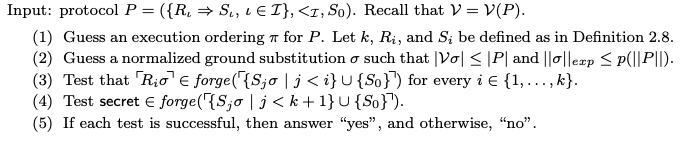
\includegraphics[scale=0.7]{assets/pic01.png}
  \caption{NP‑алгоритм для задачи INSECURE, где p обозначает полином, ограничивающий размер показателей произведений.}
  \label{fig:fig01}
\end{figure}

\begin{enumerate}[label=(\arabic*), leftmargin=0pt, labelwidth=1.5em, labelsep=0.5em, itemindent=0em]
\item Для любого сообщения \(t\) и любого конечного множества сообщений \(E\), если
$t\in\mathrm{forge}(E)\;\Longrightarrow\;\text{тогда существует корректная деривация из }E\text{ с целью }t$.

\item Если $F \;\to_{L_{oc}(t)}\;F,\,t\quad\text{и}\quad F,\,t \;\to_{L_{ad}(t)}\;F,\,t,\,a,$ то существует деривация \(D\) из \(F\) с целью \(a\), при этом 
  \(L_{d}(t)\notin D\).

\item Для любого конечного множества сообщений \(F\) с \(1\in F\), если $F\setminus\{u\}\;\to_{\mathcal{L}_{oc}(u)}\;F$, то есть \(u\) может быть получено из \(F\setminus\{u\}\) за один шаг,   тогда из $F\;\to_{\mathcal{L}_{oc}(u)}\;F,\,t$ следует $\ulcorner t[u\leftarrow1]\urcorner \;\in\;\mathrm{forge}\bigl(\ulcorner F[u\leftarrow1]\urcorner\bigr)$
  для любого сообщения \(t\).
\end{enumerate}
